\documentclass[a4paper, 12pt]{article}

\usepackage[sort&compress]{natbib}
\bibpunct{(}{)}{;}{a}{}{,} 

\usepackage{amsthm, amsmath, amssymb, mathrsfs, multirow, url, subfigure}
\usepackage{graphicx} 
\usepackage{ifthen} 
\usepackage{amsfonts}
\usepackage[usenames]{color}
\usepackage{fullpage}
\usepackage{setspace}
\usepackage{subfigure}
\usepackage{float}
\usepackage{hyperref}
\usepackage{algorithm,algpseudocode}
\usepackage{booktabs}
\usepackage{array}

%\RequirePackage[OT1]{fontenc} 
%\RequirePackage[colorlinks]{hyperref}
%\RequirePackage{hypernat}


%\numberwithin{equation}{section} 

\graphicspath{ {./images/} } 

\theoremstyle{plain} 
\newtheorem{theorem}{Theorem}
\newtheorem{corollary}{Corollary}
\newtheorem{proposition}{Proposition}
\newtheorem{lemma}{Lemma}

\def\wl{\par \vspace{\baselineskip}}
\theoremstyle{definition}
\newtheorem{defn}{Definition}

\theoremstyle{remark} 
\newtheorem{remark}{Remark}
\newtheorem{example}{Example}
\newtheorem{assumption}{Assumption}
\newtheorem{condition}{Condition}


\newcommand{\prob}{\mathsf{P}} 
\newcommand{\E}{\mathsf{E}}

\newcommand{\probhat}{\widehat{\mathsf{P}}}

\newcommand{\bel}{\mathsf{bel}}
\newcommand{\pl}{\mathsf{pl}}
\newcommand{\mpl}{\mathsf{mpl}}

\newcommand{\GG}{\mathbb{G}}
\newcommand{\bin}{{\sf Bin}}
\newcommand{\ber}{{\sf Ber}}
\newcommand{\pois}{{\sf Pois}}
\newcommand{\unif}{{\sf Unif}}
\newcommand{\nm}{{\sf N}}
\newcommand{\expo}{{\sf Exp}}
\newcommand{\gam}{{\sf Gamma}}
\newcommand{\stt}{{\sf t}}
\newcommand{\dir}{{\sf Dir}}

\newcommand{\A}{\mathcal{A}} 
\newcommand{\B}{\mathscr{B}} 
\newcommand{\RR}{\mathbb{R}}
\newcommand{\X}{\mathcal{X}} 
\newcommand{\U}{\mathcal{U}}
\newcommand{\Z}{\mathscr{Z}}
\newcommand{\XX}{\mathbb{X}}
\newcommand{\YY}{\mathbb{Y}}
\newcommand{\UU}{\mathbb{U}}
\newcommand{\VV}{\mathbb{V}}
\newcommand{\WW}{\mathbb{W}}

\newcommand{\PP}{\mathbb{P}}

\renewcommand{\L}{\mathscr{L}}

\newcommand{\G}{\mathscr{G}}
\newcommand{\Gbar}{\overline{\mathscr{G}}}
\newcommand{\gbar}{\bar{g}}

\newcommand{\Nbrack}{N_{[\,]}}
\newcommand{\Jbrack}{J_{[\,]}}

\newcommand{\avec}{\boldsymbol{a}}
\newcommand{\bvec}{\boldsymbol{b}}
\newcommand{\Bvec}{\boldsymbol{B}}
\newcommand{\dvec}{\boldsymbol{d}}
\newcommand{\evec}{\boldsymbol{e}}
\newcommand{\rvec}{\boldsymbol{r}}
\newcommand{\tvec}{\boldsymbol{t}}
\newcommand{\Tvec}{\boldsymbol{T}}
\newcommand{\uvec}{\boldsymbol{u}}
\newcommand{\Uvec}{\boldsymbol{U}}
\newcommand{\vvec}{\boldsymbol{v}}
\newcommand{\Vvec}{\boldsymbol{V}}
\newcommand{\xvec}{\boldsymbol{x}}
\newcommand{\Xvec}{\boldsymbol{X}}
\newcommand{\yvec}{\boldsymbol{y}}
\newcommand{\Yvec}{\boldsymbol{Y}}
\newcommand{\zvec}{\boldsymbol{z}}
\newcommand{\Zvec}{\boldsymbol{Z}}

\newcommand{\sign}{\mathrm{sign}}

\newcommand{\vbeta}{\boldsymbol{\beta}}
\newcommand{\veps}{\boldsymbol{\varepsilon}}
\newcommand{\veta}{\boldsymbol{\veta}}
\newcommand{\vphi}{\boldsymbol{\varphi}}
\newcommand{\vPhi}{\boldsymbol{\Phi}}
\newcommand{\vtheta}{\boldsymbol{\theta}}
\newcommand{\vxi}{\boldsymbol{\xi}}
\newcommand{\vSigma}{\boldsymbol{\Sigma}}
\newcommand{\vzeta}{\boldsymbol{\zeta}}

\newcommand{\Amat}{\mathbf{A}}
\newcommand{\Bmat}{\mathbf{B}}
\newcommand{\Cmat}{\mathbf{C}}
\newcommand{\Dmat}{\mathbf{D}}
\newcommand{\Gmat}{\mathbf{G}}
\newcommand{\Imat}{\mathbf{I}}
\newcommand{\Lmat}{\mathbf{L}}
\newcommand{\Pmat}{\mathbf{P}}
\newcommand{\Rmat}{\mathbf{R}}
\newcommand{\Umat}{\mathbf{U}}
\newcommand{\Vmat}{\mathbf{V}}
\newcommand{\Wmat}{\mathbf{W}}
\newcommand{\Xmat}{\mathbf{X}}
\newcommand{\Zmat}{\mathbf{Z}}

\newcommand{\Xbar}{\overline{X}}
\newcommand{\xbar}{\overline{x}}
\newcommand{\Ubar}{\overline{U}}
\newcommand{\ubar}{\overline{u}}
\newcommand{\Ybar}{\bar Y}%{\overline{Y}}
\newcommand{\ybar}{\bar y}%{\overline{y}}

\renewcommand{\phi}{\varphi} 
\newcommand{\eps}{\varepsilon}

\DeclareMathOperator{\logit}{logit}


\newcommand{\iid}{\overset{\text{\tiny iid}}{\,\sim\,}}
\newcommand{\ind}{\overset{\text{\tiny ind}}{\,\sim\,}}

\title{Index matching portfolios}
\author{Robert Skowron\footnote{McKelvey School of Engineering, Washington University in St. Louis, {\tt r.skowron@wustl.edu@wustl.edu}} \quad and \quad Nicholas Syring\footnote{Department of Mathematics and Statistics, Washington University in St. Louis,  {\tt nasyring@wustl.edu.}}}
\date{\today}

\begin{document}

\maketitle



\begin{abstract}
	We review approaches to solving the sparse portfolio index tracking problem in investment management. We explore in additional depth the work of George and McCulloch (1997) and elaborate on the applications of a spike and slab variable selection process for tracking portfolios. Potential further applications of this method are discussed. Finally, we discuss the potential applications of generalized fiducial inference to the problem and areas for continued research.


\smallskip

\emph{Keywords and phrases:} Sparse portfolio, index tracking, regularization, variable selection, Bayesian inference, generalized fiducial inference, Markov chain Monte Carlo

\end{abstract}


\section{Introduction}
\label{S:intro}

Stock indices like the S\&P 500 and Russell 2000 are large, diverse groups of assets of particular relevance to investors.  However, for active managers, there are many reasons why it would not it beneficial to invest even a moderate portion of the assets in these indices. There are several reasons for this including the costs associated with holding many assets, the difficulty of managing a portfolio of many assets, and the inability to deploy excess capital to higher alpha generating bets.  Therefore investors may seek to closely replicate or track the performance of a whole index by carefully selecting a small, manageable subset of its assets and deploying excess capital to more tactical bets.

The most straightforward way to solve the index tracking problem is to pose it as an optimization problem in which one minimizes a measure of the tracking error over acceptable portfolios.  Difficulties with this approach arise if one includes practical considerations in the optimization problem such as bounds on the number of assets and amounts invested in each, which take the form of constraints; see, e.g. Fastrich et al. (2014) and Benidis et al. (2018).  These constrained optimizations often can be solved using mixed integer programming but may converge slowly for high-dimensional data.

Other approaches to index tracking involve replacing the tracking error minimization by an approximation or heuristic algorithm as in the above references or by changing the optimization criteria.  For example, a Markowitz mean-variance portfolio model that minimizes portfolio variance while achieving a minimum return can approximate index tracking when the target return is the index return; see Fastrich et al. (2015) and Puelz et al. (2018).

In contrast to optimization methods, Bayesian methods for index tracking output a range of potential portfolios rather than a single solution.  This can be beneficial as estimating a covariance matrix for a large number of correlated assets requires a significant time scale to avoid singularity or ill-condition. George and McCulloch (1997) regress index returns on asset returns and use a spike and slab type prior to encourage sparsity in the number of assets selected to remain in the model.  The marginal posterior of included assets can quantify the uncertainty in asset selection, better enabling the portfolio manager to make a final subjective judgement.  Variations on the approach in George and McCulloch (1997) involve different prior specifications of sparsity, such as the SCAD penalty of Fan and Li (2001) and the spike and slab lasso of Ročková and George (2018).  A new Bayesian-like generalized fiducial approach to sparse regression was introduced in Williams and Hannig (2019).  Rather than directly encouraging sparse portfolios, the generalized fiducial approach limits acceptable portfolios to those with only minimally correlated assets.

The paper is organized as follows. Section 2 reviews the optimization problem and various proposed methods for solving. Section 3 reviews Bayesian approaches to the same problem. Section 3 also includes an in-depth look at the spike and slab approach of George and McCulloch (1997) with a more detailed discussion of applications. Additionally, we discuss a possible way to solve the constrained optimization problem using a Dirichlet prior with reversible jump Markov chain Monte Carlo. Section 4 investigates the generalized fiducial inference (GFI) approach and discusses potential applications of such a method. Finally, the paper is concluded in section 6 with suggestions for additional avenues of future investigation.
       

\section{The Optimization Problem}

Adopting the notation of Benidis et al. (2018) let $\textbf{r}^b = (r_1^b,...,r_T^b)^\top \in \mathbb{R}^T$ and $X = [\textbf{r}_1,...,\textbf{r}_T]^\top \in \mathbb{R}^{T\times N}$ denote the returns of the index and the $N$ assets of the index over $T$ time periods.  Let $\textbf{b}\in\mathbb{R}_+^N$ denote the normalized index weights of each asset, i.e. $b^\top 1_{T\times 1} = 1$ and $X\textbf{b} = \textbf{r}^b$.  

A portfolio is defined as a weight vector $\textbf{w} = (w_1, ..., w_N)$ giving the proportion invested in each asset.  For example, when the investor is limited to long positions the portfolio satisfies $w_i \geq 0$ for every $i = 1, ..., N$ and $\textbf{w}^top 1 = 1$.  Then, the tracking error of the portfolio can be measured in many ways, the primary of which is the $L_2-$error or empirical tracking error
\[\text{ETE}(\textbf{w})=\frac{1}{T}||X\textbf{w}-\textbf{r}^b||_2^2.\]

As described in the introduction, we desire a portfolio with only a small number of assets relative to the size of the index.  However, sparse minimization of the empirical tacking error of a long portfolio is not a trivial problem. Benidis et al. (2018) defines the sparse optimization problem
\begin{align}
\text{minimize}_{\textbf{w}}& \frac{1}{T}||X\textbf{w}-\textbf{r}^b||_2^2 + \lambda||\textbf{w}||_0\nonumber\\
\text{subject to}& \textbf{w}^\top 1_{N\times 1}=1, \nonumber \\
 & \textbf{w}\geq 0_{N\times 1}.
\end{align} 
The primary challenge is the presence of the nonconvex penalty $\lambda||\textbf{w}||_0$.  Benidis et al. (2018) introduce a convex approximation to this penalty and perform the minimization using their LAIT and related procedures.  The resulting solution produces a sparse, long-only portfolio with good tracking performance.

Other potential methods of solving this problem include mixed integer programming, genetic algorithms. However, it is not possible to guarantee optimality using these methods and they often come with a considerable performance cost. Other heuristic methods can also be applied. For example, one could solve the unconstrained optimization problem and identify the most significant contributors. Then, secondary optimizations could be run with the limited set of assets and constraints can be specified as a constant per choice of assets.

Regardless of the methodology, these methods all result in singular solutions (although one could run numerous iterations while varying the sparsity parameter). Given that we are using high dimensional, correlated data, the the empirical covariance matrix can often be ill-conditioned which can result in highly sensitive results. In the next section, we discuss Bayesian methods which provide distributional results which may help alleviate some of those issues.

\section{Bayesian methods}

George and McCulloch (1997) presents methods for variable selection in regression from a Bayesian viewpoint.  A primary application is construction of index-tracking portfolios.  They begin with a regression model of the index returns
$\mathbf{r}^b = X \mathbf{w} + \mathbf{\epsilon}$
where $\mathbf{\epsilon}\sim \nm_T(0,\sigma^2I_{T\times T})$.  Such a regression model is somewhat artificial because the index returns actually are a \emph{deterministic} linear combination of the constituent asset returns.  However, since the Gaussian kernel contains the (negative) empirical tracking error, maximizing the likelihood of (a sparse version of) the model is equivalent to minimizing the empirical tracking error.  To achieve sparsity in the predictors, and hence a small portfolio, George and McCulloch (1997) consider independent Bernoulli priors of the form
\begin{align}
\pi(\gamma) = \prod_{i=1}^N\alpha_i^{\gamma_i}(1-\alpha_i)^{(1-\gamma_i)}
\end{align}
for $\alpha_i\in(0,1)$ and where $\gamma \in \{0,1\}^N$ denotes which assets are included in the portfolio. Then, conditional on such $\gamma$, the $\beta_i$ are distributed as
\begin{align}
\pi(\beta_i \vert \gamma) = (1-\gamma_i)N(0,v_{0_{\gamma_i}}) + \gamma_i N(0,v_{1_{\gamma_i}})
\end{align}
where $v_0$ and $v_1$ can be constant or varying based say on the number of non-zero gammas. For the problem at hand, this construction poses two challenges. First, it does not guarantee that $\beta_i$ will not be less than zero (i.e. a long-only constraint) and secondly, that $\sum\beta_i=1$ (i.e. no leverage constraint).

The posterior density $\pi_n(\gamma)$ given the data is proportional to the likelihood times the prior density, and can be sampled using, for instance, Metropolis-Hastings within a Gibbs sampler.

\begin{algorithm}
\caption{MCMC for spike and slab}
\begin{algorithmic}[1] 
\State $\gamma_i = 0 \forall i$
\While{$n<N$}
\State Propose a new sample of $\gamma$, call it $\gamma^\star$, by randomly drawing an index $i$ and setting $\gamma^\star_i=1-\gamma_i$
\State Compute the acceptance ratio (on the log scale):
	\[a=\log \pi_n(\gamma^\star) - \log \pi_n(\gamma^i) + \log \pi(\gamma^i) - \log \pi(\gamma^\star)\]
\State Generate $U\sim \unif(0,1)$
\If {$\exp(a)>U$}
\State Accept $\gamma^{n+1}=\gamma^\star$
\Else
\State Reject the proposed $\gamma^\star$
\EndIf
\EndWhile
\end{algorithmic}
\end{algorithm}


\subsection{Revisiting George and McCulloch (1997)}

To begin our analysis, we start by refreshing the example performed in George and McCulloch (1997) and providing some additional insights. Using the Wharton Research Data Services (WRDS) we obtain weekly returns for stocks in the S\&P 500 from January 2012 to December 2018. Following the methodology laid out in Section 6 of George and McCulloch (1997) we compute the marginal probabilities of inclusion for the stocks. Utilizing 200 randomly chosen stocks, as in their example, we can observe a similar nature of marginal inclusion probabilities where a small number are nearly always included and rapidly fall off with fewer than 50 stocks being selected more than a handful of iterations.

\begin{figure}[H]
\subfigure[Replication of 1985-1991 analysis]{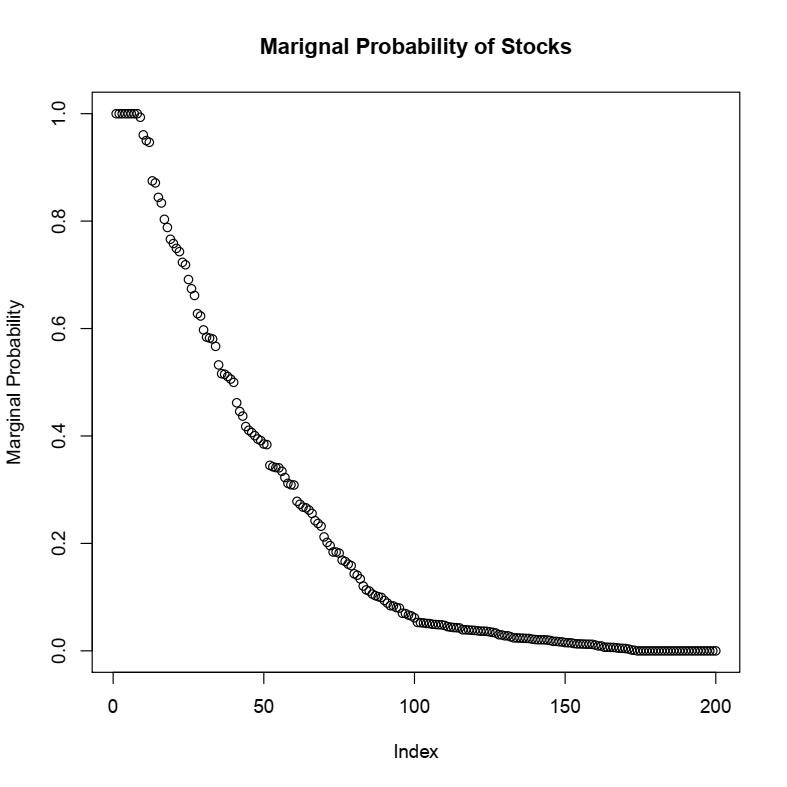
\includegraphics[width=8cm]{colmeans-plot-orig}}
\hfill
\subfigure[Algorithm applied to 2012-2018]{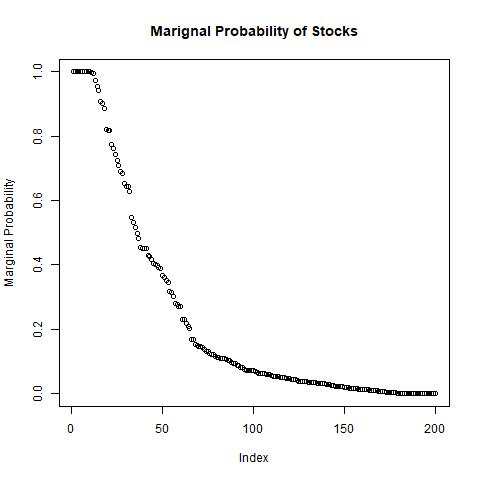
\includegraphics[width=8cm]{colmeans-plot-recent}}
\caption{Marginal probability of inclusion by applying George and McCulloch (1997) to the weekly returns for S\&P 500 from 2012-2018 }
\end{figure}

Beyond the tracking portfolio construction, there is additional information embedded in this plot. Suppose that for a certain time period, this graph depicted more candidates selected nearly always or perhaps larger gaps in inclusion probabilities. This type of information can perhaps provide context as to the State of the market. If additional candidates are selected with high frequency, that could speak to a decrease in the correlation amongst assets and thus a requirement to include additional assets for explanatory power. Likewise, large gaps could indicate consolidation in that a few assets are disproportionately responsible for the performance of the market. These secondary analysis provide lift to the Bayesian framework over the standard optimization methodologies.

The original application continues by running nested regressions and identifying the incremental explanatory power as measured by $R^2$ of each additional candidate stock. Here, we supply a different measure to demonstrate the explanatory power, tracking error, computed as $TE=\sqrt{Var(r_p-r_b)}$. We can surmise that, on the basis of in-sample tracking error, only a limited subset of stocks would be required to support a tracking error of less than 1 percent annually.

\begin{figure}[H]
\centering
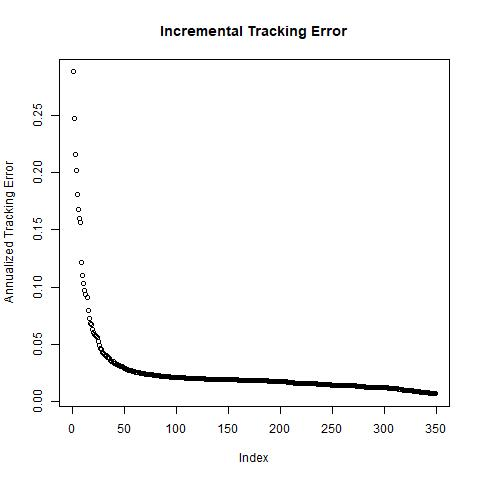
\includegraphics[width=8cm]{te-plot}
\caption{In sample results applying George and McCulloch (1997) to the weekly returns for S\&P 500 from 2012-2018. Values are computed by sequentially including assets based on marginal probability }
\end{figure}

A common follow-up question from a portfolio manager would be to ask how consistent are the results? That is, looking at those top several stocks that appear to be chosen almost always, do those remain consistent over multiple iterations? Or, particularly due to the correlation structure inherent in the stock market, do we see patterns emerge where highly correlated stocks might be chosen as equivalents? As it turns out, the top stocks selected are frequently the same. Over numerous iterations, we identify stocks such as AAPL, AMZN, BA, XOM, and MSFT being selected frequently. In George and McCulloch (1997) they explore this looking at the relative probability of individual models and finding that only a subset stand out.

However, based on those frequent selections, it begs the question of whether or not a naive approach to stock selection would do just as well. To investigate this, we use the same period of data (2012-2018) and compare both the in and out of sample performance of the spike and slab algorithm to five different naive selection methods:
\begin{itemize}
	\itemsep=0em
	\item[1.] Selecting the top 10 stocks by market cap
	\item[2.] Selecting the top stock in each GICS Sector by market cap ($\approx 10$)
	\item[3.] Selecting the top stock in each GICS Group by market cap ($\approx 25$)
	\item[4.] Selecting the top stock in each GICS Industry by market cap ($\approx 70$)
	\item[5.] Selecting the top stock in each GICS Sub-Industry by market cap ($\approx 150$)
\end{itemize}
where GICS refers to the Global Industry Classification Standard. The spike and slab algorithm is run on 250 days of data (approximately 1 year) and any stock that has a marginal inclusion probability of greater than 80\% is selected. For the same date, we construct the above naive portfolios using equal weighted contributions from the selected stocks. The portfolios are then held for 20 days (approximately 1 month) after which we rebalance the portfolios using the same logic and repeat until the end of 2018.

\begin{figure}[H]
\centering
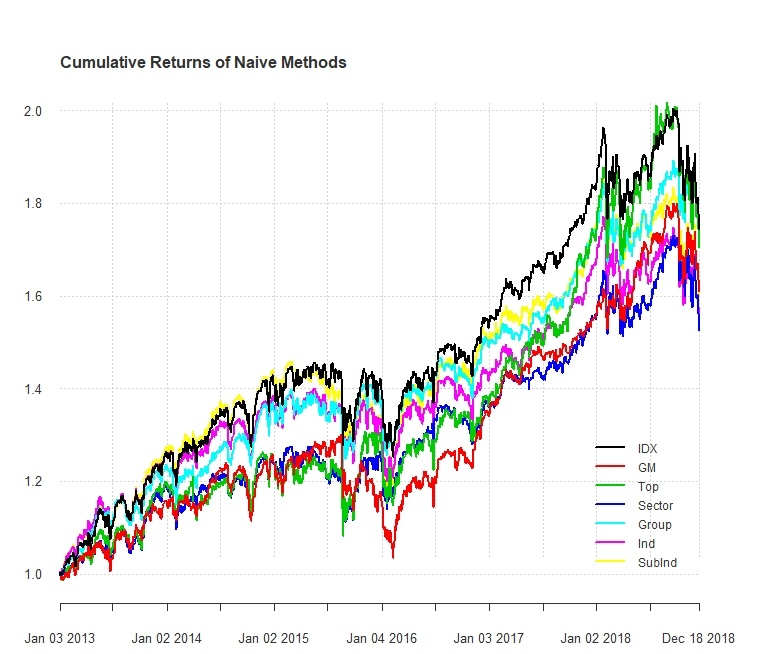
\includegraphics[width=15cm]{out-of-sample}
\caption{Comparing spike and slab to naive approaches for the weekly returns for S\&P 500 from 2012-2018}
\end{figure}

\begin{table}[H]
\caption{Tracking error and correlation comparison for spike and slab and naive methods}
\centering
\begin{center}
\begin{tabular}{lcc}
\toprule
                        & \multicolumn{1}{r}{\textbf{Tracking Error}} & \multicolumn{1}{r}{\textbf{Correlation}} \\
\midrule
\textbf{Spike and Slab} & 5.21\%                                      & .911                                     \\
\textbf{Top 10}         & 5.98\%                                      & .910                                     \\
\textbf{Sector}         & 4.80\%                                      & .925                                     \\
\textbf{Group}          & 3.72\%                                      & .956                                     \\
\textbf{Industry}       & 2.61\%                                      & .978                                     \\
\textbf{SubIndustry}    & 3.04\%                                      & .972                                    \\
\bottomrule
\end{tabular}
\end{center}
\end{table}

As can be seen by the graph and the table, the spike and slab methodology performs decently, but ultimately underperforms (in a tracking error sense) many of the naive methods.

\subsection{With constraints}
The basic hierarchical model of George and McCulloch (1997) places a normal prior on the asset weights $w$, which does not take into account any type of holding constraints, e.g. long only portfolios.  Here we present an alternative model for long-only portfolios:
\begin{align}
\textbf{r}^b &\sim \nm_{T}(X\textbf{w}, \sigma^2I_{T\times T})\\
\gamma_i &\stackrel{ind.}{\sim} \ber(\alpha_i) \\
\sigma^2 | \gamma & \sim \text{IG}(\nu/2,\,\nu\lambda_\gamma/2)\\
\textbf{w}|\gamma, \sigma^2 & \sim Dir(||\gamma||_0; \beta).
\end{align}

Here the asset weights are given a Dirichlet prior conditional on the included assets.  This prior enforces the constraints $\textbf{w}^\top 1_{N\times 1}=1$ and $\textbf{w}\geq 0_{N\times 1}$. Additionally,for the above, the proposal is Bernoulli with some high probability of $1$ if $\gamma^i_j =1$ and some low probability of $1$ if $\gamma^i_j =0$. Such a proposal will tend to slowly change the included assets. Implementing this model is difficult in practice for two reasons. First, it requires us to utilize a reversible jump MCMC in order to change candidate stock inclusions. And secondly, for the Dirichlet prior we have to accept or reject the entire space at once. This results in a low acceptance rate and thus the MCMC needs to be run over a significant number of iterations. Roughly, the algorithm is as follows:
\\
\\
\begin{algorithm}
\caption{RJMCMC with Dirichlet Prior}
\begin{algorithmic} [1]
\While{$n<N$}
\State {Run a Metropolis Hastings MCMC step a la Algorithm 1 to determine a $\beta^\star$ proposal}
\State Calculate birth, death and relocate parameters as follows
	\If {$|\beta|_0 < size$}
		\State {$birth \gets (1/3)Poisson(|\beta|_0+1,\mu)/Poisson(|\beta|_0,\mu)$}
	\Else
		\State {$birth \gets 0$}
	\EndIf
	\If {$|\beta|_0 > 1$}
		\State {$death \gets (1/3)Poisson(|\beta|_0-1,\mu)/Poisson(|\beta|_0,\mu)$}
	\Else
		\State {$death \gets 0$}
	\EndIf
	\State {$relocate \gets \max(1-b-d,0)$}
\State {Compute move probabilities $b, r, d$  from a multinomial distribution with probabilities $(birth, death, relocate)$}
\algstore{myalg}
 \end{algorithmic}
\end{algorithm}

\begin{algorithm}
\begin{algorithmic}
\algrestore{myalg}
\If {Birth: $b=1$}
	\State Choose an index $i$ that currently has $\beta_i=0$
	\State Compute the jump probability ($\eta$) of including this new covariate given the likelihood ratio of the Gaussian distributions
	\State Generate $\beta^\star$ with $\beta_i=U(0,1)$ and reduce all the non-zero $\beta_j$ proportionally
	\State Generate $U\sim \unif(0,1)$
	\If {$\eta>U$}
		\State Accept $\beta^{n+1}=\beta^\star$
	\Else
		\State Reject the proposed $\beta^\star$
	\EndIf

\ElsIf {Death: $d=1$}
	\State Choose an index $i$ that currently has $\beta_i \neq 0$
	\State Compute the jump probability ($\eta$) of excluding this covariate given the likelihood ratio of the Gaussian distributions
	\State Set $\beta^\star$ with $\beta_i=0$ and increase all the non-zero $\beta_j$ proportionally
	\State Generate $U\sim \unif(0,1)$
	\If {$\eta>U$}
		\State Accept $\beta^{n+1}=\beta^\star$
	\Else
		\State Reject the proposed $\beta^\star$
	\EndIf
\ElsIf {Relocate: $r=1$}
	\State Choose indices $i, j$ and set $\beta^\star$ with $\beta_i$ and $\beta_j$ swapped
	\State Compute the jump probability ($\eta$) of swapping these covariates given the likelihood ratio of the Gaussian distributions
	\State Generate $U\sim \unif(0,1)$
	\If {$\eta>U$}
		\State Accept $\beta^{n+1}=\beta^\star$
	\Else
		\State Reject the proposed $\beta^\star$
	\EndIf
\Else
	\State No change in $\beta$
\EndIf
\EndWhile
\end{algorithmic}
\end{algorithm}

However, while theoretically an alternative option to optimization problems, the implementation requires considerable time to converge. As an example, over several tens of thousands of iterations, if the number of candidate stocks was larger than 25 the algorithm rarely moved significantly away from equal weighting. This limitation puts this methodology out of consideration for many portfolio managers.
For more information about the reversible jump MCMC, see Hastie and Green (2012).

\section{Generalized Fiducial Inference}
Fiducial Inference is an area of statistical inference originally proposed by R.A. Fisher to attempt to find distributional representations of parameters without requiring priors. While originally dismissed due to various concerns, recent research in generalized fiducial inference (GFI) has identified some potential applications for the methods of analysis. In particular, the recent paper of Williams and Hannig (2019) makes remarks about the application of GFI to variable selection in high dimensional situations.

As they discuss in the paper, algorithms such as LASSO and SCAD require penalization functions based on the magnitude of the covariates. As in our portfolio selection problem, the ideal state would be binary inclusion (i.e. $\ell_0$) of covariates. Williams and Hanning (2019) describe their approach where the underlying premise is to identify non-zero parameters that are non-redundant in that they contain the minimal amount of information to explain or predict the observed data. These subsets of the parameter space are referred to as \textit{$\epsilon$-admissible}. Paraphrasing from the paper for explanation, suppose that there is a model space \{$x_1, x_2, ... x_p$\} are covariates and $Y \sim N(\beta_1 x_1 + \beta_2 x_2 + ... +\beta_p x_p, \sigma^2 I_p)$. If the unknown, but true values of \textbf{$\beta$} are $(b_1,b_2,0,...0)$, then the parameter space consisting of \{$x_1, x_2, x_3$\} would \textit{not} be \textit{$\epsilon$-admissible} because the subset \{$x_1, x_2$\} would perfectly predict it. The method constructs a probability distribution on such \textit{$\epsilon$-admissible} subsets providing a Bayesian-like posterior over the subsets with fewer covariates.

Certain sectors within the stock universe are highly correlated (although not necessarily collinear) and thus a methodology that strives to identify and remove models with redundancies with a true $\ell_0$ constraint would seem like a good approach to our problem. Utilizing the code provided by Mr. Williams, with some adjustments, we attempted to apply the algorithm to our 2012-2018 returns data. Our observations were that the approach did correctly narrow down to approximately 20 or so assets. However, the stocks selected were widely varying as contrasted with the George and McCulloch (1997) method that had more consistency. In all likelihood, this is due to the correlation structure of the market where one could likely find assets that are near substitutes for each other.

However, there are additional areas for future research here. First, alternative implementations of the attempts we have made here. Perhaps different hyper parameter settings for $p_0$, the number of iterations, etc. could produce fruitful results. Secondly, if the top stocks selected are indeed optimal, can we identify the related $\epsilon$-admissible subsets to use in analyzing highly correlated alternative choices? That is, do the {$\epsilon$-admissible subsets beget some information about the inherent structure of the market? Thirdly, given the fact that it does appear to accurately reduce the dimension of the problem, can this be applied as an initial filter to the standard optimization problem, similar to how we have shown as an extension of the spike and slab algorithm?

\section{Conclusion}

In this paper, we reviewed the problem and some common methods used currently in asset management to identify sparse portfolios of securities for index tracking. We refreshed the spike and slab algorithm put forth in George and McCulloch (1997) using more recent data and provided some additional insights on its performance and use cases. We also identified a methodology that would provide a solution for the constrained optimization case in RJMCMC with a Dirichlet prior. Finally, we introduced the idea of generalized fiducial inference and briefly explored its  potential utility in solving this problem. In addition to these explorations, we also note several extensions for future investigation. First, does the density or distribution of the selection probabilities from either the spike and slab algorithm or GFI algorithm provide any information about the structure of the market? Secondly, what is the utility of these types of algorithms as inputs into the standard optimization problem and does this provide an avenue of stepwise based solutions to it?

\section*{Data Availability}
All code utilized in the analysis for this paper can be found on \href{https://github.com/bob-skowron/SU19-Independent-Study}{\color{blue}Github}. Data was sourced from \href{https://wrds-web.wharton.upenn.edu/wrds/}{\color{blue}Wharton Research Data Services} via the \textit{wrds} Python package.

\section*{References}

\begin{description}

\item{} Benidis, K., Feng, Y., and Palomar, D. P.~(2018). Sparse Portfolios for High-Dimensional Financial Index Tracking. \emph{IEEE Transactions on Sigmal Processing}~66(1), 155-170.

\item{} Fan, J., and Li, R.~(2001). Variable Selection via Nonconcave Penalized Likelihood and its Oracle Properties. \emph{Journal of American Statistical Association}~96, 1348–1360.

\item{} Fastrich, B., Paterlini, S., and Winker, P.~(2014). Cardinality versus q-norm constraints for index tracking. \emph{Quantitative Finance}~14(11), 2019-2032, \\DOI: 10.1080/14697688.2012.691986

\item{} Fastrich, B., Paterlini, S. and Winker, P.~(2015). Constructing optimal sparse portfolios using regularization methods. \emph{Comput Manag Sci}~12(3) 417–434. \\https://doi.org/10.1007/s10287-014-0227-5

\item{} George, E. I., and McCulloch, R. E.~(1997). Approaches for Bayesian variable selection. \emph{Statistica Sinica}~7, 339-373.

\item{} Hastie, D. I. and Green, P. J. (2012), Model choice using reversible jump Markov chain Monte Carlo. Statistica Neerlandica, 66: 309-338. doi:10.1111/j.1467-9574.2012.00516.x

\item{} Puelz, D., Hahn, R. and Carvalho, Carlos M.~(2018). Sparse Mean-Variance Portfolios: A Penalized Utility Approach. \url{https://papers.ssrn.com/sol3/papers.cfm?abstract_id=2729504}.

\item{} Ročková, Veronika and George, Edward. (2018). The Spike-and-Slab LASSO. Journal of the American Statistical Association. 113. 10.1080/01621459.2016.1260469.

\item{} Williams, J. P., and Hannig, J.~(2019). Non-Penalized Variable Selection In High-Dimensional Linear Model Settings Via Generalized Fiducial Inference. \emph{Annals of Statistics}.~47(3), 1723-1753. 

\end{description}

\end{document}





